\documentclass[border=10pt]{standalone}
\usepackage[svgnames]{xcolor}
\usepackage{amsmath}
\usepackage{pgfplots}
\pgfplotsset{compat=newest}
\usepackage[sfdefault]{FiraSans}
\usepackage{FiraMono}
\renewcommand*\familydefault{\sfdefault}
\begin{document}
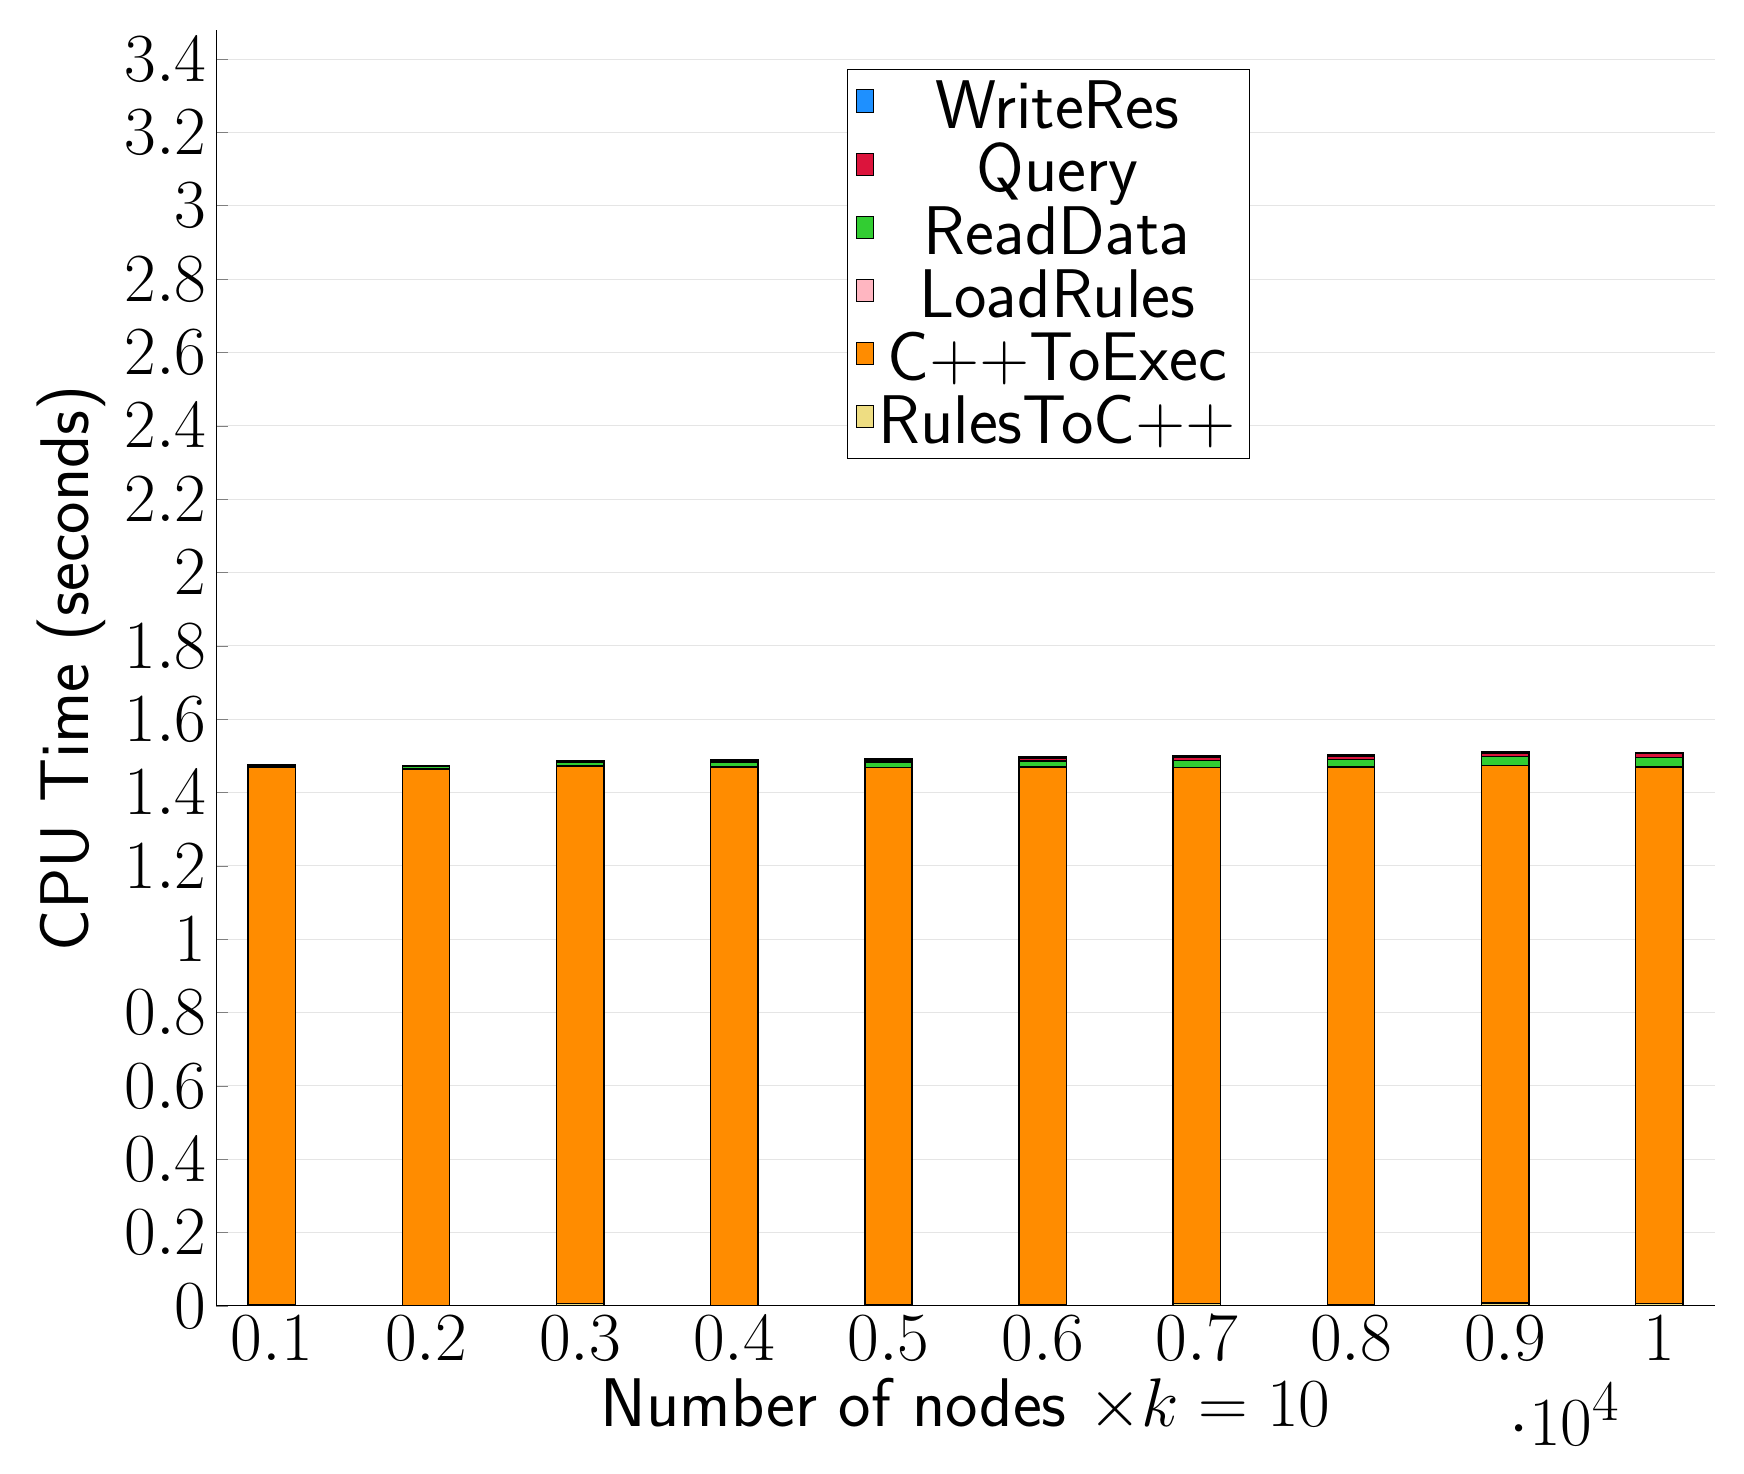
\begin{tikzpicture}
\begin{axis}[
   ybar stacked,
   width=1.7\textwidth,
   bar width=0.6cm,
   ymajorgrids, tick align=inside,
   major grid style={draw=gray!20},
   xtick=data,
   ymin=0, ymax=3.4779999999999998,
   axis x line*=bottom,
   axis y line*=left,
   enlarge x limits=0.04,
   legend style={
       at={(0.69, 0.97)},
       anchor=north east,
       legend columns=1,
       font=\Huge,
   },
   ylabel={CPU Time (seconds)},
   xlabel={Number of nodes $\times k=10$},
   label style={font=\Huge},
   tick label style={font=\Huge},
]
\addlegendimage{fill=DodgerBlue, draw=black, line width=0.2pt}
\addlegendentry{WriteRes}
\addlegendimage{fill=Crimson, draw=black, line width=0.2pt}
\addlegendentry{Query}
\addlegendimage{fill=LimeGreen, draw=black, line width=0.2pt}
\addlegendentry{ReadData}
\addlegendimage{fill=LightPink, draw=black, line width=0.2pt}
\addlegendentry{LoadRules}
\addlegendimage{fill=DarkOrange, draw=black, line width=0.2pt}
\addlegendentry{C++ToExec}
\addlegendimage{fill=LightGoldenrod, draw=black, line width=0.2pt}
\addlegendentry{RulesToC++}
\addplot +[fill=LightGoldenrod, draw=black, line width=0.55pt] coordinates {
(1000, 0.0020000000000000005)
(2000, 0.0)
(3000, 0.006000000000000001)
(4000, 0.0)
(5000, 0.004000000000000001)
(6000, 0.004000000000000001)
(7000, 0.006000000000000001)
(8000, 0.0020000000000000005)
(9000, 0.008000000000000002)
(10000, 0.006000000000000001)
};
\addplot +[fill=DarkOrange, draw=black, line width=0.55pt] coordinates {
(1000, 1.468)
(2000, 1.464)
(3000, 1.466)
(4000, 1.47)
(5000, 1.464)
(6000, 1.4659999999999997)
(7000, 1.462)
(8000, 1.468)
(9000, 1.466)
(10000, 1.464)
};
\addplot +[fill=LightPink, draw=black, line width=0.55pt] coordinates {
(1000, 0.0001538)
(2000, 0.00014359999999999997)
(3000, 0.0001608)
(4000, 0.0001548)
(5000, 0.00015979999999999998)
(6000, 0.00015020000000000002)
(7000, 0.0001656)
(8000, 0.000157)
(9000, 0.00015)
(10000, 0.0001518)
};
\addplot +[fill=LimeGreen, draw=black, line width=0.55pt] coordinates {
(1000, 0.0036458)
(2000, 0.006354)
(3000, 0.0095072)
(4000, 0.012687799999999999)
(5000, 0.014790399999999999)
(6000, 0.0164132)
(7000, 0.0193182)
(8000, 0.020308)
(9000, 0.023471400000000003)
(10000, 0.025407000000000002)
};
\addplot +[fill=Crimson, draw=black, line width=0.55pt] coordinates {
(1000, 0.0014572)
(2000, 0.0025206)
(3000, 0.004229)
(4000, 0.004694)
(5000, 0.006256599999999999)
(6000, 0.007191400000000001)
(7000, 0.0084206)
(8000, 0.0087794)
(9000, 0.0094808)
(10000, 0.010449799999999999)
};
\addplot +[fill=DodgerBlue, draw=black, line width=0.55pt] coordinates {
(1000, 0.0008618)
(2000, 0.0010382)
(3000, 0.0017202000000000003)
(4000, 0.0020222)
(5000, 0.00229)
(6000, 0.0025908000000000003)
(7000, 0.0028786000000000003)
(8000, 0.0029268)
(9000, 0.0032782000000000006)
(10000, 0.0033824)
};
\end{axis}
\end{tikzpicture}

\end{document}
